% !TeX root = main.tex
% !TEX program = pdflatex

% =============================================================
% CAPÍTULO 12 — ESQUELETO (pendiente de redactar)
% Capítulo de cierre/síntesis del curso. Mapea con RA5 (Acotar el error de
% medida cometido en un sistema de instrumentación y adquisición de datos)
% y RA8 (Diseñar un sistema de instrumentación completo, desde sensor y
% acondicionador hasta adquisición y visualización, elaborando un plan
% coherente para resolver la situación planteada).
% Este capítulo NO introduce teoría nueva: recopila y aplica los
% "presupuestos de errores" (Error Budget) ya vistos sueltos en cada
% familia de sensores (caps. 3, 4, 6, 7) sobre 1-2 casos de estudio
% completos, de principio a fin.
% =============================================================

\chapter{Integración y Diseño de Sistemas de Instrumentación}\label{cap:integracion}

El recorrido de este libro ha ido bloque a bloque: primero el sensor y sus principios físicos, después el acondicionamiento de su señal, luego la digitalización, la defensa frente al ruido, la transmisión y, por último, el programa que lee y registra. Un sistema de instrumentación real, sin embargo, no es esa lista: es un conjunto de decisiones que se toman a la vez y que se condicionan unas a otras. La resolución del convertidor tiene que justificarse frente al ruido de la etapa anterior; la ganancia del amplificador depende del margen que admita la entrada del convertidor; la distancia a la que está el sensor puede obligar a cambiar la forma de transmitir la señal; y el tiempo que se dedica a medir decide cuánto ruido se puede promediar. El hilo que ata todas esas decisiones es cuantitativo y es el mismo que abría el libro: la incertidumbre que la medida final necesita tener.

Este capítulo no introduce teoría nueva: recopila y aplica. Sus dos primeras secciones son el método: cómo se ordena el diseño de un sistema completo (Sección~\ref{sec:metodologia_diseno}) y cómo se comprueba que el conjunto cumple la especificación, sumando las contribuciones de error de todos los bloques (Sección~\ref{sec:presupuesto_global}). Las dos siguientes ponen ese método a prueba sobre dos sistemas completos: uno del laboratorio de comunicaciones ópticas (Sección~\ref{sec:caso_fibra}) y otro de la instrumentación industrial (Sección~\ref{sec:caso_temperatura}).

La lección que se repite en ambos casos conviene anunciarla desde ahora, porque es la que más cuesta interiorizar: el error dominante de un sistema de medida no siempre está en el sensor. Con frecuencia está en el convertidor, en el amplificador o en lo que el entorno acopla por el camino, y averiguar cuál de ellos manda es, precisamente, el resultado del presupuesto de errores~\cite{jcgm100_2008_gum,taylor1997erroranalysis}.

\section{Metodología de Diseño de un Sistema de Instrumentación}\label{sec:metodologia_diseno}

Todo diseño de instrumentación empieza por una especificación, y una especificación útil es numérica. La pregunta que la abre no es ``¿qué sensor pongo?'', sino ``¿para qué se mide?'': qué decisión tiene que permitir tomar la medida, en qué márgenes tiene que ser válida y, sobre todo, con cuánta incertidumbre. De ahí salen los cuatro números que gobiernan el resto del diseño: el \emph{rango} que hay que cubrir, la \emph{incertidumbre máxima} admisible, la \emph{banda} o velocidad de respuesta que exige el fenómeno --que incluye desde la frecuencia más alta de la señal hasta el tiempo que se puede dedicar a promediar-- y el \emph{entorno} en que la medida debe sobrevivir. Cuando esa especificación no la fija el cliente ni una norma, el ingeniero tiene que fijarla él mismo antes de tocar un componente, y escribirla; un diseño sin especificación escrita no puede validarse ni discutirse, solo defenderse con opiniones.

\marginnote{\textbf{Las preguntas de la especificación:} ¿qué decisión permite tomar la medida y con cuánta incertidumbre? ¿en qué rango de la magnitud? ¿a qué velocidad hay que responder, o cuánto tiempo se puede promediar? ¿en qué entorno electromagnético y climático va a vivir? ¿durante cuánto tiempo, con qué mantenimiento y con qué presupuesto? Si alguna de estas respuestas no existe, el diseño que venga después será una apuesta.}

A partir de ahí, el diseño avanza en el orden que muestra la Figura~\ref{fig:flujo_diseno}, con una etapa por cada decisión y un criterio claro para tomarla, resumido en la Tabla~\ref{tab:decisiones_diseno}. Se elige el \emph{sensor} por el principio físico más adecuado al mensurando, atendiendo a su sensibilidad, a su ruido propio y a su deriva; se diseña el \emph{acondicionamiento} para llevar la señal al margen que admite la entrada del convertidor, filtrando la banda que no interesa y cuidando la carga que se le presenta al sensor; se elige la \emph{digitalización} por la resolución útil y la velocidad necesarias, no por el número de bits del catálogo; se decide la \emph{transmisión y la protección} según la distancia, el entorno electromagnético y las exigencias normativas; y se organiza la \emph{lectura y el registro} pensando en quién va a consumir el dato y en cómo va a documentarse. La última etapa, la \emph{validación}, no es un bloque del sistema, sino la comprobación de que los demás encajan: la suma de sus errores, hecha como se explica en la Sección~\ref{sec:presupuesto_global}, debe caber en la incertidumbre que pedía la especificación.

\begin{table}[ht]
    \centering
    \small
    \setlength{\tabcolsep}{3pt}
    \forceversofloat % la tabla cae en página par (verso); sin forzar, el caption sale al lado contrario
    \begin{tabularx}{\linewidth}{@{} >{\raggedright\arraybackslash}p{0.24\linewidth} >{\centering\arraybackslash}X >{\centering\arraybackslash}X @{}}
        \toprule
        \textbf{Decisión} & \textbf{Qué la determina} & \textbf{Dónde se estudia} \\
        \midrule
        Fijar la especificación & El uso de la medida: qué decisión debe permitir y con qué incertidumbre, rango y banda & Capítulo~\ref{cap:metrologia} \\
        Elegir el sensor & El principio físico adecuado, su sensibilidad, su ruido propio y su deriva & Capítulos~\ref{cap:resistivos} a~\ref{cap:opticos} \\
        Diseñar el acondicionamiento & Llevar la señal al margen del convertidor y limitar la banda a la de la medida & Capítulo~\ref{cap:opamps} \\
        Elegir la digitalización & La resolución útil y la velocidad necesarias & Capítulo~\ref{cap:daq} \\
        Decidir transmisión y protección & La distancia, el entorno electromagnético y las exigencias normativas & Capítulos~\ref{cap:ruido} y~\ref{cap:buses} \\
        Organizar lectura y registro & Quién consume el dato, en qué formato y con qué trazabilidad & Capítulo~\ref{cap:instrumentacion_virtual} \\
        Validar el conjunto & El presupuesto de errores frente a la especificación & Capítulo~\ref{cap:metrologia} y Sección~\ref{sec:presupuesto_global} \\
        \bottomrule
    \end{tabularx}
    \caption[Decisiones de diseño y el criterio que las determina.]{Las decisiones de un diseño de instrumentación, el criterio que las determina y el capítulo donde se estudia cada una. El orden es el de la figura anterior y también el de la responsabilidad: fijar mal la especificación arruina el diseño entero, y ningún componente posterior puede compensarlo.}\label{tab:decisiones_diseno}
\end{table}

\begin{marginfigure}
    \centering
    \begin{tikzpicture}[scale=0.8, >=Stealth]
        % ── cadena de decisiones ──────────────────────────────
        \draw[thick] (1.0,6.1) rectangle (4.6,6.8);
        \node[font=\scriptsize] at (2.8,6.55) {especificación};
        \node[gray, font=\tiny] at (2.8,6.28) {(magnitud, rango, $u$, banda, entorno)};
        \draw[thick] (1.0,5.15) rectangle (4.6,5.85);
        \node[font=\scriptsize] at (2.8,5.6) {sensor};
        \node[gray, font=\tiny] at (2.8,5.33) {Capítulos~\ref{cap:resistivos} a~\ref{cap:opticos}};
        \draw[thick] (1.0,4.2) rectangle (4.6,4.9);
        \node[font=\scriptsize] at (2.8,4.65) {acondicionamiento};
        \node[gray, font=\tiny] at (2.8,4.38) {Capítulo~\ref{cap:opamps}};
        \draw[thick] (1.0,3.25) rectangle (4.6,3.95);
        \node[font=\scriptsize] at (2.8,3.7) {digitalización};
        \node[gray, font=\tiny] at (2.8,3.43) {Capítulo~\ref{cap:daq}};
        \draw[thick] (1.0,2.3) rectangle (4.6,3.0);
        \node[font=\scriptsize] at (2.8,2.75) {transmisión y protección};
        \node[gray, font=\tiny] at (2.8,2.48) {Capítulos~\ref{cap:ruido} y~\ref{cap:buses}};
        \draw[thick] (1.0,1.35) rectangle (4.6,2.05);
        \node[font=\scriptsize] at (2.8,1.8) {validación del error};
        \node[gray, font=\tiny] at (2.8,1.53) {Capítulo~\ref{cap:metrologia} y Sección~\ref{sec:presupuesto_global}};
        % enlaces descendentes
        \foreach \y in {6.1,5.15,4.2,3.25,2.3} {
            \draw[->] (2.8,\y) -- (2.8,\y-0.25);
        }
        % bucle de iteración
        \draw[->] (1.0,1.7) -- (0.5,1.7) -- (0.5,5.5) -- (0.97,5.5);
        \node[gray, font=\tiny, rotate=90] at (0.28,3.6) {si no cabe, se repite};
    \end{tikzpicture}
    \caption[Orden de las decisiones en el diseño de un sistema de medida.]{Orden de las decisiones en el diseño de un sistema de instrumentación y, a la izquierda, el camino de vuelta. La especificación abre el proceso y la validación lo cierra comprobando que el presupuesto de errores cabe en ella; cuando no cabe, se revisan las decisiones anteriores en orden inverso --primero la banda y el rango, después el convertidor, y solo al final el sensor, que es lo más caro de cambiar--.}\label{fig:flujo_diseno}
\end{marginfigure}

Dos consecuencias de este orden merecen destacarse, porque son las que distinguen un diseño meditado de un montaje. La primera es que el proceso es \emph{iterativo}: si al llegar a la validación el presupuesto no cabe, lo barato es volver atrás y ajustar la banda o el rango --medir más despacio, promediar más, aceptar un margen menor--, y solo al final cambiar el sensor, que es lo que más cuesta en dinero, en tiempo y en trabajo ya hecho. La segunda es que la resolución que se pide al convertidor no puede ser mayor que la que la etapa anterior es capaz de sostener: si el ruido del acondicionamiento equivale a un milivoltio, tener veinte bits de convertidor no mejora nada, porque los últimos dígitos serán ruido. Determinar cuántos bits resultan de verdad útiles --el número efectivo de bits del Capítulo~\ref{cap:daq}-- es justamente el cálculo que cierra el diseño, y es lo primero que se comprueba en el presupuesto de errores de la sección siguiente.

\marginnote{\textbf{El error más frecuente:} confundir resolución con exactitud. Un convertidor de veinticuatro bits ofrece veinticuatro bits de \emph{resolución}, pero la exactitud de la medida la fijan el sensor, la referencia, el ruido y la calibración. Escribir ``resolución de 24 bits'' en una especificación que exige una incertidumbre del \SI{0.1}{\percent} no demuestra nada; el presupuesto de errores, en cambio, sí.}

\section{El Presupuesto de Errores de Extremo a Extremo}\label{sec:presupuesto_global}

Los capítulos anteriores han ido dejando presupuestos de error parciales: el de los sensores resistivos (Sección~\ref{sec:errores_resistivos}), el de los reactivos (Sección~\ref{sec:errores_reactivos}), el de las imperfecciones del acondicionamiento (Sección~\ref{sec:errores_opamp}) y el de los sensores ópticos (Sección~\ref{sec:errores_opticos}), más el número efectivo de bits del convertidor (Sección~\ref{sec:enob}) y el ruido que el entorno acopla por el camino (Sección~\ref{sec:acoplamientos}). Lo que falta, y es el objeto de esta sección, es el paso de la parte al todo: un presupuesto que conteste si el sistema completo cumple la especificación y, sobre todo, cuál de sus bloques manda.

El método tiene tres pasos. El primero es \emph{referir todas las contribuciones a la entrada}, es decir, expresarlas en unidades del mensurando y no en las del punto donde aparecen: una tensión de \emph{offset} de \SI{100}{\micro\volt} en un amplificador de ganancia mil es un décimo de milivoltio en su salida, pero hay que dividirla además por la sensibilidad del sensor para saber a cuántos grados o a cuántos vatios equivale. Cada contribución se convierte así mediante su coeficiente de sensibilidad, que es exactamente lo que hace la fórmula de propagación de la incertidumbre del Capítulo~\ref{cap:metrologia}. El segundo paso es \emph{clasificar} cada contribución: las aleatorias e independientes se combinan en cuadratura, mientras que las sistemáticas no se compensan entre sí y hay que sumarlas algebraicamente en el peor caso, salvo la parte que la calibración corrija. El tercero es \emph{combinar y comparar} con la especificación. Para contribuciones aleatorias e independientes, la incertidumbre combinada es la raíz de la suma de los cuadrados,
\begin{equation}\label{eq:presupuesto_global}
    u_c = \sqrt{\sum_{i} u_i^2}
\end{equation}
donde cada $u_i$ es ya la contribución de un bloque referida a la entrada~\cite{taylor1997erroranalysis}, igual que en el presupuesto parcial de los sensores resistivos (ecuación~\eqref{eq:error_budget}), pero ahora con todos los bloques de la cadena a la vez. La Tabla~\ref{tab:contribuciones_error} recoge esas contribuciones y la forma de referir cada una a la entrada.

\begin{table}[ht]
    \centering
    \small
    \setlength{\tabcolsep}{3pt}
    \forcerectofloat % la tabla cae en página impar (recto); sin forzar, el caption sale al lado contrario
    \begin{tabularx}{\linewidth}{@{} >{\raggedright\arraybackslash}p{0.25\linewidth} >{\centering\arraybackslash}X >{\centering\arraybackslash}X @{}}
        \toprule
        \textbf{Bloque} & \textbf{Contribución típica} & \textbf{Cómo se refiere a la entrada} \\
        \midrule
        Sensor & Sensibilidad y su tolerancia, no linealidad, histéresis y deriva térmica & Dividiendo por su sensibilidad (Secciones~\ref{sec:errores_resistivos}, \ref{sec:errores_reactivos} y~\ref{sec:errores_opticos}) \\
        Excitación o referencia & Tolerancia y estabilidad de la corriente o de la tensión de excitación & Dividiendo por la sensibilidad, o por la relación de excitación \\
        Acondicionamiento & Tensión de \emph{offset}, error de ganancia, CMRR y ruido propio & Dividiendo por la ganancia y por la sensibilidad (Sección~\ref{sec:errores_opamp}) \\
        Convertidor & Cuantización y ruido real, medido por su ENOB & Escalando por el fondo de escala y dividiendo por la sensibilidad (Sección~\ref{sec:enob}) \\
        Interferencia & Tensiones inducidas, bucles de tierra y ruido acoplado & Dividiendo por la sensibilidad, con el ancho de banda en juego (Sección~\ref{sec:acoplamientos}) \\
        Transmisión & Error del lazo de corriente o del canal digital & Del fondo de escala en el lazo; nulo si el dato ya es digital (Sección~\ref{sec:lazo_420}) \\
        Calibración & Incertidumbre del patrón y del procedimiento & Igual que el bloque al que corrige (Capítulo~\ref{cap:metrologia}) \\
        \bottomrule
    \end{tabularx}
    \caption[Contribuciones al presupuesto de errores de un sistema completo.]{Contribuciones que hay que tener presentes en un presupuesto de extremo a extremo y la forma de referirlas a la entrada. La lista es la de los capítulos anteriores puesta en columna: si alguna falta, el presupuesto está incompleto por pequeño que sea su valor.}\label{tab:contribuciones_error}
\end{table}

Un ejemplo numérico muestra por qué este cálculo es más útil de lo que parece. Supóngase un sistema con cinco contribuciones aleatorias, expresadas todas en porcentaje del fondo de escala: el sensor, con su no linealidad y su histéresis, aporta un \SI{0.20}{\percent}; la referencia de excitación, un \SI{0.10}{\percent}; la interferencia acoplada por el cableado, otro \SI{0.10}{\percent}; el acondicionamiento, un \SI{0.05}{\percent}; y el convertidor, un \SI{0.024}{\percent} correspondiente a doce bits efectivos. La ecuación~\eqref{eq:presupuesto_global} da una incertidumbre combinada de \SI{0.25}{\percent}, que cabe con holgura en una especificación del \SI{0.50}{\percent} (Figura~\ref{fig:presupuesto_barras}). Lo interesante no es eso, sino el reparto: el sensor concentra el \SI{63}{\percent} de la varianza total, de modo que es ahí donde hay que invertir el esfuerzo. Duplicar la resolución del convertidor apenas cambiaría nada --dejaría la incertidumbre combinada en \SI{0.2503}{\percent}--, mientras que reducir a la mitad la no linealidad del sensor la bajaría a \SI{0.18}{\percent}.

\begin{marginfigure}
    \centering
    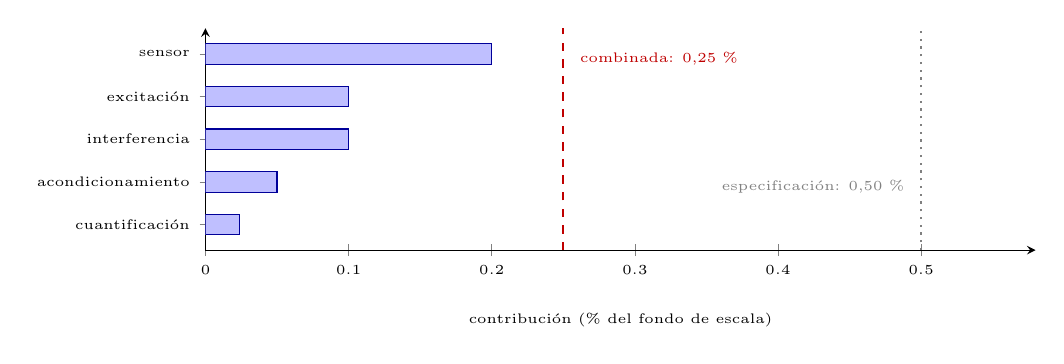
\begin{tikzpicture}
        \begin{axis}[
            width=\linewidth, height=4.4cm,
            xbar, bar width=0.26cm,
            xmin=0, xmax=0.58, ymin=-0.6, ymax=4.6,
            ytick={0,1,2,3,4},
            yticklabels={cuantificación,acondicionamiento,interferencia,excitación,sensor},
            yticklabel style={font=\tiny},
            xtick={0,0.1,0.2,0.3,0.4,0.5},
            xticklabel style={font=\tiny},
            font=\scriptsize,
            axis lines=left,
            xlabel={contribución (\% del fondo de escala)},
            every axis x label/.style={at={(0.5,-0.24)}, anchor=north, font=\tiny},
        ]
            \addplot[fill=blue!25, draw=blue!60!black] coordinates {
                (0.024,0) (0.05,1) (0.10,2) (0.10,3) (0.20,4)};
            \draw[dashed, thick, red!75!black] (axis cs:0.25,-0.6) -- (axis cs:0.25,4.6);
            \node[red!75!black, font=\tiny, anchor=south west] at (axis cs:0.255,3.5) {combinada: 0,25 \%};
            \draw[dotted, thick, gray] (axis cs:0.50,-0.6) -- (axis cs:0.50,4.6);
            \node[gray, font=\tiny, anchor=south east] at (axis cs:0.495,0.5) {especificación: 0,50 \%};
        \end{axis}
    \end{tikzpicture}
    \caption[Ejemplo de presupuesto de errores de un sistema completo.]{Ejemplo de presupuesto de extremo a extremo con cinco contribuciones aleatorias referidas a la entrada. La línea roja marca la incertidumbre combinada --\SI{0.25}{\percent}, muy cerca de la mayor de las contribuciones-- y la línea gris de puntos, el límite que impone la especificación. La conclusión se lee en las barras: el sensor concentra el \SI{63}{\percent} de la varianza, así que mejorar el convertidor no serviría de nada.}\label{fig:presupuesto_barras}
\end{marginfigure}

\marginnote{\textbf{Detalles que deciden un presupuesto:} (1)~el convertidor se juzga por su número efectivo de bits y no por los nominales, porque el ENOB ya incluye su ruido real; (2)~las contribuciones sistemáticas no se combinan en cuadratura, sino que se suman en el peor caso salvo la parte que la calibración elimine; (3)~las magnitudes de influencia --temperatura, tensión de alimentación, humedad-- hay que contarlas aparte de las condiciones de referencia; y (4)~buena parte de los errores que arruinan una medida no están en el sensor, sino en la referencia de excitación y en lo que el cable recoge por el camino.}

La consecuencia de todo lo anterior es una regla de trabajo que conviene repetir porque es contraintuitiva: \emph{en un presupuesto de errores solo merece la pena mejorar el término que domina}. La raíz de la suma de los cuadrados se parece mucho al mayor de sus sumandos --en el ejemplo, \SI{0.25}{\percent} frente a \SI{0.20}{\percent}--, de modo que reducir a la mitad una contribución que ocupa el tercer lugar no cambia el resultado de forma apreciable, mientras que atacar la dominante lo cambia de inmediato. La traducción presupuestaria es directa: un convertidor con más bits, un amplificador de mejores prestaciones o un blindaje más caro solo mejoran la medida si su bloque es el que manda. Y la traducción de diseño es la de la sección anterior: el presupuesto se calcula al final del proceso, pero es su árbitro desde el principio, porque es el que decide si la especificación se cumple y dónde hay que gastar el esfuerzo.

\section{Caso de Estudio 1: Medida de Potencia Óptica en un Enlace de Fibra}\label{sec:caso_fibra}

El primer sistema que se diseña de principio a fin en este capítulo es el de la especificación siguiente: medir la potencia óptica media que llega al extremo de un enlace de fibra monomodo a \SI{1550}{\nano\meter}. El caso reúne los ingredientes del laboratorio de comunicaciones ópticas de este curso --un detector semiconductor del Capítulo~\ref{cap:opticos}, una etapa de transimpedancia y un convertidor del Capítulo~\ref{cap:daq}-- y añade la exigencia de registrar la medida desde el puesto de control, que es lo que lo convierte en un buen ejemplo de integración con los Capítulos~\ref{cap:buses} y~\ref{cap:instrumentacion_virtual}.

\subsection{La Especificación}\label{sub:fibra_especificacion}

La medida tiene que cubrir de 0 a \SI{100}{\micro\watt} (de 0 a $-10$~dBm) de potencia óptica media, con una incertidumbre objetivo del \SI{2}{\percent} de la lectura --unos \SI{0.09}{\decibel}--, y ha de responder hasta \SI{1}{\kilo\hertz}, porque la fuente puede estar modulada y interesa medir la potencia media de la modulación. El detector y su electrónica estarán en el banco, junto al extremo de la fibra, y el registro se hará de forma automática desde un ordenador situado a unos metros, con la fecha, la identificación del módulo y la fecha de su última calibración. Hay que tener presente, además, que el error relativo admisible es sobre la lectura: el caso más exigente no es el fondo de escala, sino el extremo inferior del rango útil, donde el mismo error absoluto pesa mucho más.

\subsection{Del Fotodiodo al Convertidor}\label{sub:fibra_sensor}

A \SI{1550}{\nano\meter} el silicio ya no responde --su banda prohibida deja de absorber por encima de unos \SI{1100}{\nano\meter}--, así que el detector ha de ser de un material de banda prohibida más estrecha: un fotodiodo de InGaAs, con una responsividad de unos \qty{0.9}{A/W}, una corriente de oscuridad de unos \SI{5}{\nano\ampere} y una capacidad de unión de unos \SI{10}{\pico\farad}. Los tres números importan: el primero fija la conversión de potencia en corriente (ecuación~\eqref{eq:responsividad}), el segundo limita la medida en el fondo del rango y el tercero condiciona la estabilidad de la etapa siguiente. En el extremo inferior de la especificación, una potencia de \SI{1}{\micro\watt} produce una corriente de \SI{0.9}{\micro\ampere}: el sistema tiene que ser capaz de medir con precisión una corriente de ese orden.

La conversión de esa corriente en una tensión la hace un amplificador de transimpedancia, la misma etapa que se presentó al estudiar los detectores ópticos (Figura~\ref{fig:tia_pd}) y que es la versión para corriente del amplificador de carga del Capítulo~\ref{cap:opamps}. Con la tierra virtual del operacional, toda la corriente del fotodiodo circula por la resistencia de realimentación, de modo que la tensión de salida es
\begin{equation}\label{eq:fibra_transferencia}
    V_{out} = R_f \cdot I_{ph} = R_f \cdot \mathcal{R} \cdot P
\end{equation}
y basta elegir la resistencia para que el fondo de escala llene casi todo el margen del convertidor. Con $R_f = \SI{22}{\kilo\ohm}$ y \SI{100}{\micro\watt} de entrada, la corriente es \SI{90}{\micro\ampere} y la salida \SI{1.98}{\volt}: un valor que entra con holgura en la referencia de \SI{2.048}{\volt} que se elige para el convertidor, dejando un pequeño margen para la corriente de oscuridad y las tolerancias. El condensador de realimentación $C_f$, de unos \SI{2}{\pico\farad}, no es un adorno: compensa la capacidad del fotodiodo para que el lazo no oscile y, de paso, limita la banda, que es la primera palanca para reducir el ruido. La Figura~\ref{fig:fibra_bloques} recoge la cadena completa con sus valores.

\begin{marginfigure}
    \centering
    \begin{tikzpicture}[scale=0.8, >=Stealth]
        \draw[thick] (0.8,5.4) rectangle (4.4,6.15);
        \node[font=\scriptsize] at (2.6,5.9) {fotodiodo InGaAs};
        \node[gray, font=\tiny] at (2.6,5.63) {$\mathcal{R} = \SI{0.9}{A/W}$, $I_d = \SI{5}{\nano\ampere}$};
        \draw[thick] (0.8,4.4) rectangle (4.4,5.15);
        \node[font=\scriptsize] at (2.6,4.9) {transimpedancia};
        \node[gray, font=\tiny] at (2.6,4.63) {$R_f = \SI{22}{\kilo\ohm}$, $C_f = \SI{2}{\pico\farad}$};
        \draw[thick] (0.8,3.4) rectangle (4.4,4.15);
        \node[font=\scriptsize] at (2.6,3.9) {convertidor};
        \node[gray, font=\tiny] at (2.6,3.63) {16 bits, \SI{2.048}{\volt}, \SI{10}{\kilo\hertz}};
        \draw[thick] (0.8,2.4) rectangle (4.4,3.15);
        \node[font=\scriptsize] at (2.6,2.9) {módulo con interfaz};
        \node[gray, font=\tiny] at (2.6,2.63) {USB o Ethernet, calibrado};
        \foreach \y in {5.4,4.4,3.4} {
            \draw[->] (2.6,\y) -- (2.6,\y-0.25);
        }
        \draw[->] (2.6,6.9) -- (2.6,6.17) node[midway, right, font=\scriptsize] {$P$};
        \draw[->] (2.6,2.4) -- (2.6,1.9) node[midway, right, font=\tiny, anchor=west] {SCPI};
        \node[gray, font=\tiny, anchor=north] at (2.6,1.85) {PC: lectura y registro con PyVISA};
    \end{tikzpicture}
    \caption[Cadena del medidor de potencia óptica del primer caso de estudio.]{Cadena completa del medidor de potencia óptica, con los valores elegidos en cada etapa. La etapa de transimpedancia va en el mismo encapsulado que el fotodiodo, porque el nodo entre ambos es el punto de mayor impedancia del sistema; el módulo entrega la medida ya calibrada por su interfaz digital, y el ordenador se limita a leerla y registrarla.}\label{fig:fibra_bloques}
\end{marginfigure}

\marginnote{\textbf{Dónde va el amplificador:} entre el fotodiodo y la entrada del operacional hay un nodo de impedancia altísima y con muy poca corriente: es el peor punto del sistema para tender un cable. Alargarlo añadiría capacidad parásita --que degrada la banda y desestabiliza la etapa, como se vio al estudiar la capacidad de unión (ecuación~\eqref{eq:capacidad_union})-- y lo convertiría en una antena. Por eso la decisión de transmisión de los Capítulos~\ref{cap:ruido} y~\ref{cap:buses} se resuelve aquí dentro del propio módulo: la señal que viaja por el cable es ya digital.}

\subsection{Digitalización y Lectura}\label{sub:fibra_digitalizacion}

El tamaño del convertidor no se decide en el fondo de escala, donde todo cabe, sino en el extremo inferior del rango, que es donde el error relativo aprieta. Con 16 bits y una referencia de \SI{2.048}{\volt}, el escalón es de \SI{31.25}{\micro\volt}, que referido a la entrada con la relación~\eqref{eq:fibra_transferencia} equivale a \SI{1.58}{\nano\watt}: sobre una lectura de \SI{1}{\micro\watt} supone un \SI{0.16}{\percent}, holgadamente por debajo del \SI{2}{\percent} exigido; con 12 bits el escalón sería dieciséis veces mayor --\SI{25}{\nano\watt}-- y el error de cuantización se acercaría al \SI{2.5}{\percent}, incumpliendo la especificación por sí solo. La resolución se pide, por tanto, desde el peor caso de la lectura y no desde el catálogo. En cuanto a la velocidad, una banda de \SI{1}{\kilo\hertz} exige muestrear por encima del doble de esa frecuencia; \SI{10}{\kilo\hertz} deja margen para el filtro de antialiasing del Capítulo~\ref{cap:opamps} y simplifica su diseño. El ruido, por último, no es el problema de este sistema: sumando el ruido térmico de $R_f$, el de disparo del fotodiodo y el del propio amplificador en la banda de trabajo, el conjunto equivale a menos del \SI{0.02}{\percent} de una lectura de \SI{1}{\micro\watt}, dos órdenes de magnitud por debajo de las contribuciones de exactitud.

El conjunto se encapsula como un medidor de potencia con salida digital: el microcontrolador del módulo aplica el factor de calibración, resta la corriente de oscuridad y expone la medida por USB o por Ethernet, de modo que el ordenador del puesto de control la lee con el mismo diálogo SCPI de la Sección~\ref{sec:scpi} y el mismo guion de Python de la Sección~\ref{sec:pyvisa} --pedir la identificación, comprobar que el instrumento responde y leer la potencia--, registrando además la fecha de la última calibración que el propio módulo publica. Es el sensor inteligente de la Sección~\ref{sec:smart_sensors} aplicado a un instrumento óptico: la calibración viaja dentro del equipo.

\subsection{El Presupuesto de Errores del Sistema}\label{sub:fibra_presupuesto}

Con el método de la Sección~\ref{sec:presupuesto_global}, el presupuesto del medidor se organiza en torno a un hecho decisivo: la mayor parte de sus errores son de ganancia y se eliminan calibrando el módulo contra un patrón trazable, de modo que lo que queda después de la calibración son las derivas y las no linealidades que la calibración no puede absorber, más las contribuciones aleatorias. La Tabla~\ref{tab:fibra_presupuesto} recoge todas ellas referidas al extremo inferior del rango útil, que es donde las contribuciones relativas son mayores.

\begin{table}[ht]
    \centering
    \small
    \setlength{\tabcolsep}{3pt}
    \forceversofloat % la tabla cae en página par (verso); sin forzar, el caption sale al lado contrario
    \begin{tabularx}{\linewidth}{@{} >{\raggedright\arraybackslash}p{0.34\linewidth} >{\centering\arraybackslash}X >{\centering\arraybackslash}X >{\centering\arraybackslash}X @{}}
        \toprule
        \textbf{Contribución} & \textbf{Valor} & \textbf{Tipo} & \textbf{Cómo se reduce} \\
        \midrule
        Incertidumbre de la calibración del módulo & \SI{1.0}{\percent} & Sistemática & Patrón de mayor calidad y calibración periódica \\
        Deriva térmica de la responsividad y de $R_f$ & \SI{0.3}{\percent} & Sistemática & Estabilizar la temperatura del módulo \\
        No linealidad del módulo en el rango & \SI{0.2}{\percent} & Sistemática & Calibración en varios puntos \\
        Corriente de oscuridad residual & \SI{0.2}{\percent} & Aleatoria & Ajuste de cero y control térmico \\
        Cuantización del convertidor & \SI{0.16}{\percent} & Aleatoria & No procede: ya está muy por debajo \\
        Interferencia acoplada y zumbido de red & \SI{0.05}{\percent} & Aleatoria & Blindaje y amplificador junto al detector \\
        Ruido del amplificador y de disparo & \SI{0.02}{\percent} & Aleatoria & Reducir la banda \\
        \bottomrule
    \end{tabularx}
    \caption[Presupuesto de errores del medidor de potencia óptica.]{Presupuesto de errores del medidor de potencia óptica, con los valores referidos al extremo inferior del rango útil (lecturas de \SI{1}{\micro\watt}), que es donde cada contribución pesa más. Las tres primeras son de ganancia y las absorbe la calibración; las cuatro siguientes son lo que queda después de calibrar.}\label{tab:fibra_presupuesto}
\end{table}

Combinando los tres términos sistemáticos por suma algebraica --en el peor caso, porque se suman sin compensarse-- se obtiene un \SI{1.5}{\percent}; los cuatro aleatorios, combinados en cuadratura, aportan un \SI{0.26}{\percent}. El total en el peor caso es, por tanto, un \SI{1.76}{\percent}, y tratando todas las contribuciones como independientes el resultado baja a un \SI{1.1}{\percent}: la especificación del \SI{2}{\percent} se cumple en ambos supuestos, aunque con poco margen en el primero. El reparto es lo que más enseña del caso: la contribución dominante es la incertidumbre de la calibración --es decir, la calidad del patrón--, no el fotodiodo, ni el amplificador, ni el convertidor. Si la especificación se apretara al \SI{1}{\percent}, ningún convertidor de más bits ayudaría: habría que mejorar la referencia y estabilizar la temperatura, que es exactamente lo que anuncia la hoja de características de cualquier medidor de potencia óptico real, donde se especifican la incertidumbre de calibración y el coeficiente de temperatura y no se menciona, en cambio, el número de bits del convertidor interno.

\section{Caso de Estudio 2: Monitorización de Temperatura con Salida 4-20 mA}\label{sec:caso_temperatura}

El segundo caso mira al otro extremo del curso: es una medida industrial, con el sensor en campo, a un centenar de metros del puesto de control, y en un entorno electromagnético hostil. La magnitud es una temperatura y el objetivo no es un experimento de laboratorio, sino una medida que tiene que estar funcionando todos los días y avisar cuando algo va mal. El caso recorre la sonda de platino del Capítulo~\ref{cap:resistivos}, el transmisor de campo del Capítulo~\ref{cap:buses}, el lazo de corriente y su canal digital y, por último, las protecciones del Capítulo~\ref{cap:ruido}.

\subsection{La Especificación}\label{sub:temperatura_especificacion}

Hay que medir la temperatura de un circuito de proceso entre \SI{0}{\celsius} y \SI{200}{\celsius} con una incertidumbre de $\pm$\SI{1}{\celsius}, es decir, el \SI{0.5}{\percent} del margen de medida, y hay que hacerlo con la sonda instalada en el proceso y el sistema de control a unos \SI{150}{\meter} de distancia. Se pide además poder consultar el estado del instrumento y cambiar su rango sin desmontarlo, y que la medida sobreviva al entorno: la instalación comparte recorrido con motores y contactores, y el cableado entra en un edificio donde hay transitorios y descargas.

\subsection{Del Sensor al Transmisor de Campo}\label{sub:temperatura_sensor}

Entre los dos candidatos del capítulo de sensores de temperatura --la sonda de platino y el termopar-- la elección la decide la exactitud requerida: un termopar es más barato y cubre cientos de grados más (Sección~\ref{sec:termopares}), pero su sensibilidad es de decenas de microvoltios por grado y exige compensar la unión fría; una sonda Pt100, con su coeficiente de \SI{0.385}{\ohm\per\degreeCelsius} definido por la norma \emph{IEC 60751}, entrega una señal mucho mayor y es la opción habitual cuando se busca precisión en este rango. En una sonda de clase A, la tolerancia intrínseca llega a $\pm$\SI{0.55}{\celsius} a \SI{200}{\celsius}~\cite{iec60751_2008}: un valor que incumpliría por sí solo la especificación y que, sin embargo, no entra en el presupuesto tal cual, porque la calibración del conjunto lo elimina; lo que quedará es la incertidumbre de esa calibración.

La decisión que define la arquitectura de este caso es dónde se lee la sonda. Si se llevara su resistencia hasta el puesto de control por un par de cobre de \SI{150}{\meter}, los dos hilos de ida y vuelta sumarían unos \SI{10.5}{\ohm}, que divididos por la sensibilidad de la sonda equivalen a \textbf{\SI{27}{\celsius}} de error: un disparate. Es exactamente el problema de la conexión a 2 hilos que se estudió en el Capítulo~\ref{cap:resistivos}, pero agravado por la distancia. La solución industrial es la misma que en el caso anterior: llevar la electrónica junto al sensor. Un \emph{transmisor de campo} montado en el cabezal de la sonda la excita con una corriente pequeña, mide su resistencia con conexión de tres hilos --de modo que la resistencia de los hilos se cancela--, digitaliza el valor, aplica la linealización de la curva de platino y convierte el resultado en una corriente de \SI{4}{\milli\ampere} a \SI{20}{\milli\ampere} que representa de \SI{0}{\celsius} a \SI{200}{\celsius} (Figura~\ref{fig:temperatura_bloques}). A partir de ahí, lo que viaja por el cable ya no es una resistencia frágil ni una tensión pequeña, sino una corriente robusta.

\begin{marginfigure}
    \centering
    \begin{tikzpicture}[scale=0.8, >=Stealth]
        \draw[thick] (0.5,5.4) rectangle (4.5,6.15);
        \node[font=\scriptsize] at (2.5,5.9) {sonda Pt100, 3 hilos};
        \node[gray, font=\tiny] at (2.5,5.63) {clase A, \SI{0.385}{\ohm\per\degreeCelsius}};
        \draw[thick] (0.5,4.4) rectangle (4.5,5.15);
        \node[font=\scriptsize] at (2.5,4.9) {transmisor de campo};
        \node[gray, font=\tiny] at (2.5,4.63) {16 bits, \SI{4}{mA} a \SI{20}{mA} y HART};
        \draw[dashed, thick] (0.5,3.4) rectangle (4.5,4.15);
        \node[font=\scriptsize] at (2.5,3.9) {par trenzado apantallado};
        \node[gray, font=\tiny] at (2.5,3.63) {\SI{150}{\meter}, protecciones en los bornes};
        \draw[thick] (0.5,2.4) rectangle (4.5,3.15);
        \node[font=\scriptsize] at (2.5,2.9) {receptor del lazo};
        \node[gray, font=\tiny] at (2.5,2.63) {$R_s = \SI{250}{\ohm}$, ADC de 12 bits};
        \draw[thick] (0.5,1.4) rectangle (4.5,2.15);
        \node[font=\scriptsize] at (2.5,1.9) {controlador y registro};
        \node[gray, font=\tiny] at (2.5,1.63) {HART: diagnóstico y configuración};
        \foreach \y in {5.4,4.4,3.4,2.4} {
            \draw[->] (2.5,\y) -- (2.5,\y-0.25);
        }
        \draw[->] (2.5,6.9) -- (2.5,6.17) node[midway, right, font=\scriptsize] {$T$};
        \node[gray, font=\tiny, anchor=north] at (2.5,1.35) {alimentación de \SI{24}{\volt} por el mismo par};
    \end{tikzpicture}
    \caption[Cadena del lazo de temperatura del segundo caso de estudio.]{Cadena del lazo de temperatura. La sonda se lee con tres hilos en el propio cabezal, de modo que la resistencia de los hilos no introduce error; el transmisor digitaliza, linealiza y convierte la medida en corriente de \SI{4}{mA} a \SI{20}{mA}, que es lo que recorre los \SI{150}{\meter} de par trenzado apantallado. En el receptor, una resistencia de \SI{250}{\ohm} convierte esa corriente en una tensión de \SI{1}{\volt} a \SI{5}{\volt} que el convertidor puede leer, y el canal HART comparte el mismo par para consultar el instrumento.}\label{fig:temperatura_bloques}
\end{marginfigure}

Un par de comprobaciones cierran el diseño del sensor. La primera es el autocalentamiento: con una corriente de excitación de \SI{0.5}{\milli\ampere}, la sonda disipa unas decenas de microwatios, que con la constante de disipación de una vaina industrial se traducen en una milésima de grado, despreciable frente al presupuesto (Sección~\ref{subsec:autocalentamiento}). La segunda es la resolución del convertidor interno del transmisor, que con 16 bits sobre el margen de \SI{200}{\celsius} da escalones de tres milésimas de grado: no hay problema por ese lado. Lo que sí importa es que el transmisor se calibra junto con su sonda, porque es el conjunto --no cada pieza por separado-- lo que se contrasta contra el patrón.

\subsection{El Lazo y su Protección}\label{sub:temperatura_lazo}

El lazo que sale del transmisor se diseña con las reglas del Capítulo~\ref{cap:buses}: su presupuesto de tensión admite hasta \SI{600}{\ohm} de carga total, y este lazo carga los \SI{10.5}{\ohm} del cable más los \SI{250}{\ohm} de la resistencia de lectura, es decir, unos \SI{260}{\ohm}, de modo que al transmisor le quedan casi \SI{19}{\volt} de los \SI{24}{\volt} de alimentación, muy por encima de los \SI{12}{\volt} que necesita para regular (Sección~\ref{sub:presupuesto_lazo}). Sobre ese mismo par viaja el canal HART, que es el que permite leer los diagnósticos del instrumento y cambiar su rango desde el puesto de control sin desmontarlo (Sección~\ref{sec:hart}).

La parte que no aparece en un esquema ideal es la protección, y en este caso es imprescindible. El lazo es la antena más larga del sistema: sus \SI{150}{\meter} de cable recorren una instalación con motores y contactores (Sección~\ref{sec:acoplamientos}), y sus bornes son el punto de entrada de las descargas y los transitorios que llegan del exterior (Sección~\ref{sec:esd}). El diseño sigue las tres reglas del Capítulo~\ref{cap:ruido}: el par va trenzado y apantallado, con la malla conectada en un solo extremo para no crear un bucle de tierra (Sección~\ref{sec:tierras}); el receptor filtra la banda que no le interesa, que además es lo que separa la medida analógica de los tonos del canal digital (Sección~\ref{sec:filtrado_emi}); y en los bornes del transmisor y de la entrada se colocan diodos de protección que derivan a tierra la energía de un transitorio antes de que alcance la electrónica (Tabla~\ref{tab:comparativa_esd}).

\subsection{El Presupuesto de Errores del Sistema}\label{sub:temperatura_presupuesto}

El presupuesto de este caso, recogido en la Tabla~\ref{tab:temperatura_presupuesto}, tiene un reparto muy distinto al del medidor óptico, y de ahí su interés. La electrónica --transmisor, lazo y receptor-- aporta unas cuatro décimas de grado en el peor caso, mientras que el término dominante no está en ningún componente: está en cómo se instala la sonda en el proceso.

\begin{table}[ht]
    \centering
    \small
    \setlength{\tabcolsep}{3pt}
    \forceversofloat % la tabla cae en página par (verso); sin forzar, el caption sale al lado contrario
    \begin{tabularx}{\linewidth}{@{} >{\raggedright\arraybackslash}p{0.34\linewidth} >{\centering\arraybackslash}X >{\centering\arraybackslash}X >{\centering\arraybackslash}X @{}}
        \toprule
        \textbf{Contribución} & \textbf{Valor} & \textbf{Tipo} & \textbf{Cómo se reduce} \\
        \midrule
        Instalación: inmersión y contacto térmico & \SI{0.50}{\celsius} & Sistemática & Profundidad de inmersión y pasta conductora \\
        Calibración del conjunto sonda y transmisor & \SI{0.20}{\celsius} & Sistemática & Patrón de mayor calidad \\
        Linealidad de la sonda y del transmisor & \SI{0.10}{\celsius} & Sistemática & Calibración en varios puntos \\
        Deriva térmica del transmisor en campo & \SI{0.10}{\celsius} & Sistemática & Transmisor con bajo coeficiente ambiental \\
        Ruido e interferencia acoplados al lazo & \SI{0.05}{\celsius} & Aleatoria & Apantallamiento y filtrado del receptor \\
        Resolución del receptor tras la lectura & \SI{0.05}{\celsius} & Aleatoria & Convertidor de más bits \\
        Autocalentamiento de la sonda & \SI{0.002}{\celsius} & Sistemática & Corriente de excitación pequeña \\
        \bottomrule
    \end{tabularx}
    \caption[Presupuesto de errores del lazo de temperatura.]{Presupuesto de errores del lazo de temperatura, con todas las contribuciones referidas a la temperatura medida. La tolerancia propia de la sonda según su clase no figura en la tabla porque la absorbe la calibración del conjunto; lo que sí figura es la incertidumbre que queda después de calibrar.}\label{tab:temperatura_presupuesto}
\end{table}

La suma algebraica de los cinco términos sistemáticos da \SI{0.90}{\celsius}, y la combinación en cuadratura de los dos aleatorios, \SI{0.07}{\celsius}: el total en el peor caso es \SI{0.97}{\celsius} y, tratando todas las contribuciones como independientes, \SI{0.56}{\celsius}. La especificación de $\pm$\SI{1}{\celsius} se cumple en ambos supuestos, pero el margen del peor caso es estrecho, y ahí está la lección del caso: la mitad del presupuesto --y el término que decide si se cumple o no-- corresponde a la instalación de la sonda, no al instrumento. Un transmisor diez veces mejor no cambiaría nada; mejorar la inmersión, el contacto térmico o el aislamiento de la vaina, sí. Es la misma conclusión que en el medidor óptico, con otro protagonista: allí mandaba el patrón de calibración, aquí manda el montaje, y en ninguno de los dos casos mandaba el convertidor.

\marginnote{\textbf{Los tres presupuestos, comparados:} en el medidor óptico dominaba la calibración (el patrón); en el lazo de temperatura domina la instalación (la inmersión de la sonda); y en un sistema rápido y de bajo nivel, como los estudiados en los capítulos de sensores y ruido, lo que domina es el ruido del acondicionamiento y la interferencia. La conclusión es siempre la misma y es la del Capítulo~\ref{cap:integracion}: \textbf{el error dominante hay que buscarlo caso por caso, y casi nunca está donde la intuición lo sitúa}.}

\section{Resumen}\label{sec:conclusiones_curso}

Este capítulo, y con él el libro, se cierra volviendo al principio: a la idea de que medir es comparar una magnitud con un patrón y expresar el resultado con su incertidumbre~\cite{jcgm200_2012_vim}. Todo lo demás que se ha estudiado son los medios para hacerlo bien --y para saber cuánto de bien se está haciendo--:

\begin{itemize}
    \item \emph{Medir es cuantificar con incertidumbre} (Capítulos~\ref{cap:metrologia} y~\ref{cap:caracteristicas_sistemas_medida}): un número sin incertidumbre no es una medida, y las características estáticas y dinámicas de un sistema --sensibilidad, linealidad, histéresis, ancho de banda-- son la forma de describirlo antes de usarlo.
    \item \emph{La cadena empieza en el sensor} (Capítulos~\ref{cap:resistivos} a~\ref{cap:opticos}): cada familia de sensores aporta un principio físico distinto y, con él, un conjunto propio de errores, sensibilidades cruzadas y condicionantes de acondicionamiento. Elegir el sensor es elegir qué errores se van a tener que combatir después.
    \item \emph{La señal se prepara y se digitaliza} (Capítulos~\ref{cap:opamps} y~\ref{cap:daq}): el acondicionamiento adapta el margen y la banda, y el convertidor fija la frontera entre los dos mundos; su resolución útil la determina el ruido que le llega, no su número de bits (Sección~\ref{sec:enob}).
    \item \emph{La señal viaja y se defiende} (Capítulos~\ref{cap:ruido} a~\ref{cap:buses}): el ruido intrínseco se minimiza, la interferencia se elimina con blindaje, tierras y filtrado, y la distancia se cubre con corriente, con un lazo de \SI{4}{\milli\ampere} a \SI{20}{\milli\ampere} o con un bus; los buses de campo y los sensores inteligentes añaden, además, la información que la señal analógica no puede llevar.
    \item \emph{El software forma parte del sistema} (Capítulo~\ref{cap:instrumentacion_virtual}): la instrumentación virtual y programable multiplica las medidas, su repetibilidad y su trazabilidad, y convierte el procedimiento en algo escrito; a cambio, hay que tratarla con el mismo rigor que al resto de la cadena.
    \item \emph{El diseño se cierra con un presupuesto} (este capítulo): la especificación ordena las decisiones, el presupuesto de errores las valida y los dos casos de estudio --el medidor óptico y el lazo de temperatura-- demuestran que el error dominante no está siempre donde se espera: en uno mandaba la calibración, en el otro la instalación, y en ninguno el convertidor.
\end{itemize}

\marginnote{\textbf{La lección final:} un sistema de medida no vale por la exactitud que promete en un catálogo, sino por la incertidumbre que es capaz de demostrar y por la información que es capaz de comunicar. Eso --y no un componente concreto-- es lo que distingue una medida de un número.}
